\documentclass{llncs}

\usepackage[utf8]{inputenc}
\usepackage[brazil]{babel}

\usepackage{proof}
\usepackage{amsmath}
\usepackage{amssymb}
\usepackage{graphicx}
\usepackage{skak}

\sloppy

\begin{document}

\title{Prevenção de Ataques de Não-Terminação baseados em
Estouros de Precisão}

\author{Raphael Ernani Rodrigues and Fernando Magno Quintão Pereira}

\institute{Departamento de Ciência da Computação -- UFMG -- Brasil
\email{\{raphael,fernando\}@dcc.ufmg.br}
}


\maketitle

%mmmmmmmmmmmmmmmmmmmmmmmmmmmmmmmmmmmmmmmmmmmmmmmmmmmmmmmmmmmmmmmmmmmmmmmmmmmmmm
\begin{abstract}
Dizemos que um programa é vulnerável a um ataque de não terminação quando
um adversário pode lhe fornecer valores de entrada que façam algum de seus laços 
iterar para sempre.
A prevenção de ataques desse tipo é difícil, pois eles não se originam de bugs 
que infringem a semântica da linguagem em que o programa foi feito.
Ao contrário, essas vulnerabilidades têm origem na aritmética modular inteira de 
linguagens como C, C++ e Java, a qual possui semântica bem definida.
Neste artigo nós apresentamos uma ferramenta que detecta tais problemas, 
e que saneia código vulnerável.
A detecção da vulnerabilidade dá-se via uma análise de fluxo de informação;
a sua cura decorre de guardas que nosso compilador insere no código vulnerável.
Nós implementamos esse arcabouço em LLVM, um compilador de qualidade industrial, 
e testa-mo-no em um conjunto de programas que compraz mais de
2.5 milhões de linhas de código escrito em C.
Descobrimos que, em média, caminhos em que informação perigosa trafega são 
pequenos, sendo compostos por não mais que 10 instruções assembly.
A instrumentação que inserimos para prevenir ataques de não terminação aumenta o 
tamanho do programa saneado em cerca de 5\% em média, e torna-os menos que 2\% 
mais lentos.
\end{abstract}

%mmmmmmmmmmmmmmmmmmmmmmmmmmmmmmmmmmmmmmmmmmmmmmmmmmmmmmmmmmmmmmmmmmmmmmmmmmmmmm
\begin{abstract}
We say that a program is vulnerable to a non-termination attack if (i) it
contains a loop that is bounded by values coming from public inputs, and (ii)
an adversary can manipulate these values to force this loop to iterate forever.
Preventing this kind of attack is difficult because they do not originate
from bugs that break the semantics of the programming
language, such as buffer overflows.
Instead, they usually are made possible by the wrapping integer arithmetics
used by C, C++ and Java-like languages, which have well-defined semantics.
In this paper we present the diagnosis and the cure for this type of attack.
Firstly, we describe a tainted-flow analysis that detects non-termination
vulnerabilities.
Secondly, we provide a compiler transformation that inserts arithmetic guards on
loop conditions that may not terminate due to integer overflows.
We have implemented our framework in the LLVM compiler, and have tested it on
a benchmark suite containing over 2.5 million lines of C code.
We have found out that the typical path from inputs to loop conditions is,
on the average, less than 10 instructions long.
Our instrumentation that prevents this kind of attacks adds less than 5\%
extra code on the secured program.
The final, protected code, is, on the average, less than 2\% slower than the
original, unprotected program.
\end{abstract}

%mmmmmmmmmmmmmmmmmmmmmmmmmmmmmmmmmmmmmmmmmmmmmmmmmmmmmmmmmmmmmmmmmmmmmmmmmmmmmm
\section{Introdução}
\label{sec:int}

Um ataque de Negação de Serviços ({\em Denial-of-Service -- DoS}) consiste
em sobrecarregar um servidor com uma quantidade de falsas requisições grande o
suficiente para lhe comprometer a capacidade de atender contatos
legítimos.
Existem hoje diversas maneiras diferentes de detectar e reduzir a efetividade
desse tipo de ataque~\cite{Moore06}.
Neste artigo, contudo, descreveremos uma forma de negação de serviço que é de
difícil detecção: {\em os ataques de não-terminação}.
Um adversário realiza um ataque desse tipo fornecendo ao programa alvo entradas
cuidadosamente produzidas para forçar iterações eternas sobre um laço
vulnerável.
Um ataque de não terminação demanda conhecimento do código fonte do sistema
a ser abordado.
Não obstante tal limitação, esse tipo de ataque pode ser muito efetivo,
pois bastam algumas requisições para comprometer o sistema alvo.
Uma vez que essa quantidade de incursões é pequena, os métodos tradicionais
de detecção de negação de serviço não podem ser usados para reconhecer ataques
de não-terminação.
Além disso, dada a vasta quantidade de código aberto usado nos mais diversos
ramos da indústria de {\em software}, usuários maliciosos têm a sua
disposição um vasto campo de ação.

A detecção de código vulnerável a ataques de não-terminação é difícil.
Tal dificuldade existe, sobretudo, porque esse tipo de ataque não decorre de
deficiências de tipagem fraca, normalmente presentes em programas escritos em
C ou C++.
Programas escritos em linguagens fortemente tipadas, como Java, por exemplo,
também apresentam a principal fonte de vulnerabilidades a ataques de
não terminação: a {\em aritmética modular inteira}.
Em outras palavras, uma operação como \texttt{a + 1}, em Java, C ou C++, pode
resultar em um valor menor que aquele inicialmente encontrado na variável
\texttt{a}.
Esse fenômeno ocorrerá quando a variável \texttt{a} guardar o maior inteiro
presente em cada uma dessas linguagens.
Nesse caso, ao fim da operação, \texttt{a + 1} representará o menor inteiro
possível em complemento de dois.
Em outras palavras, um laço como \texttt{for (i = 0; i <= N; i++)} nunca
terminará se \texttt{N} for \texttt{MAX\_INT}, o maior inteiro da linguagem.

Este artigo traz duas contribuições relacionadas a ataques de não-terminação.
Em primeiro lugar, ele descreve uma técnica que descobre vulnerabilidades
relacionadas a esse tipo de ataque.
Em segundo lugar, o artigo mostra como código pode ser protegido contra tais
ataques.
A nossa técnica de detecção de vulnerabilidades é baseada em análise de
fluxo contaminado.
Tal análise é parte do arcabouço teórico de rastreamento de informação
inicialmente proposto por Denning e Denning nos anos setenta~\cite{Denning77}.
Um ataque de fluxo contaminado pode ser efetivo somente em programas cujas
operações críticas dependam de dados de entrada.
Em nosso contexto, uma operação crítica é o teste de controle de laço.
Em conjunto com o algoritmo de detecção de vulnerabilidades, nós propomos
também uma técnica para sanear programas contra ataques de não-terminação.
Nossa estratégia consiste na inserção de verificações sobre as
operações aritméticas realizadas pelo programa alvo.
Essas verificações ocorrem durante a execução do programa, e invocam código de
segurança sempre que estouros de precisão em variáveis inteira são percebidos.
Nós instrumentamos somente código que controla o número de iterações em laços.
Consequentemente, o arcabouço que propomos incorre em uma perda de
desempenho muito pequena, e, em nossa opinião, completamente justificável em
decurso do benefício que assegura.

Nós implementamos todas as idéias que discutimos neste artigo em LLVM,
um compilador de qualidade industrial~\cite{Lattner04}.
Na seção~\ref{sec:exp} descreveremos uma série de experimentos que
validam nossa análise.
Ao analisar os programas presentes na coleção SPEC CPU 2006, fomos capazes
de descobrir XX laços que são influenciados por dados provenientes de
entradas públicas, isto é, que podem ser manipuladas por um adversário.
Dentre esses laços, pelo menos XX estão sujeitos à não terminação.
Para obter esse número, utilizamos um padrão muito simples: procuramos por
laços cujo teste de parada é do tipo \texttt{i <= N}, sendo \texttt{N}
dependente da entrada.
Uma vez que nos atemos a esse tipo de condição de parada, especulamos que
a quantidade de laços vulneráveis presente nos programas de SPEC CPU 2006
seja bem maior que o valor que apuramos.
A nossa instrumentação -- usada para impedir os ataques de não-terminação --
mostra-se extremamente eficiente.
Os testes que inserimos antes de cada operação aritmética que pode levar a
um ataque de não terminação custa-nos uma perda de desempenho de menos que
XX\%.

%mmmmmmmmmmmmmmmmmmmmmmmmmmmmmmmmmmmmmmmmmmmmmmmmmmmmmmmmmmmmmmmmmmmmmmmmmmmmmm
\section{Ataques de Não-Terminação}
\label{sec:bkg}

De acordo com Appel e Palsberg~\cite[p.376]{Appel02}, um laço natural é um
conjunto de nodos $S$ do grafo de fluxo de controle (CFG) de um programa,
includindo um nodo cabeçalho $H$, com as seguintes três propriedades:
%
\begin{itemize}
\item a partir de qualquer nodo em $S$ existe um caminho que chega a $H$;
\item existe um caminho de $H$ até qualquer nodo que faz parte de $S$;
\item qualquer caminho de um nodo fora de $S$ para um nodo em $S$
contém $H$.
\end{itemize}
%
A {\em condição de parada} de um laço é uma expressão booleana
$E = f(e_1, e_2, \ldots, e_n)$, sendo cada $e_j, 1 \leq j \leq n$ um valor que
contribui para a computação de $E$.
Seja $P$ um programa que possui um laço $L$ limitado por uma condição
de parada $E = f(e_1, e_2, \ldots, e_n)$.
Dizemos que $P$ é vulnerável a um ataque de não
terminação quando as duas condições abaixo são verdadeiras sobre ele:
\begin{enumerate}
\item existe um subconjunto $E' \subseteq \{e_1, e_2, \ldots, e_n\}$ de
valores que dependem de um conjunto $I = \{i_1, i_2, \ldots, i_m\}$ de
dados lidos a partir da entrada do programa.
\item existe uma atribuição de valores $i_1 \mapsto v_1,
i_2 \mapsto v_2, \ldots, i_m \mapsto v_m$ que, ao influenciar $E'$, faz com
que o laço $L$ não termine.
\end{enumerate}
Note que a nossa definição de vulnerabilidade de não-terminação requer a
noção de dependência de dados.
Se um programa $P$ possui uma instrução que usa a variável $u$ e define a
variável $v$, então $v$ {\em depende} de $u$.
Dependências de dados são transitivas, e embora possam ser cíclicas, não
são necessariamente comutativas.

Ilustraremos ataques de não terminação via o programa mostrado na
Figura~\ref{fig:fact}(a).
Esse programa calcula o fatorial de um número inteiro na linguagem C.
O padrão que rege essa linguagem de programação não determina o tamanho do
tipo \texttt{int}.
Essa informação depende da implementação do compilador usado.
Entretanto, é usual que inteiros sejam representados como números de 32
bits em complemento de dois. 
Nesse caso, o maior inteiro representável é
$\mathit{MAX\_INT} = 2^{31} - 1 = 2,147,483,647$.
Se o parâmetro \texttt{n} for igual a $\mathit{MAX\_INT}$, então a condição
da linha 4 sempre será verdadeira, e o laço nunca terminará.
A não-terminação ocorre porque quando \texttt{i} finalmente chega a
$\mathit{MAX\_INT}$, a soma $i + 1$ nos retorna o menor inteiro possível, isto
é, $- 2^{31}$.

\begin{figure}[t!]
\begin{center}
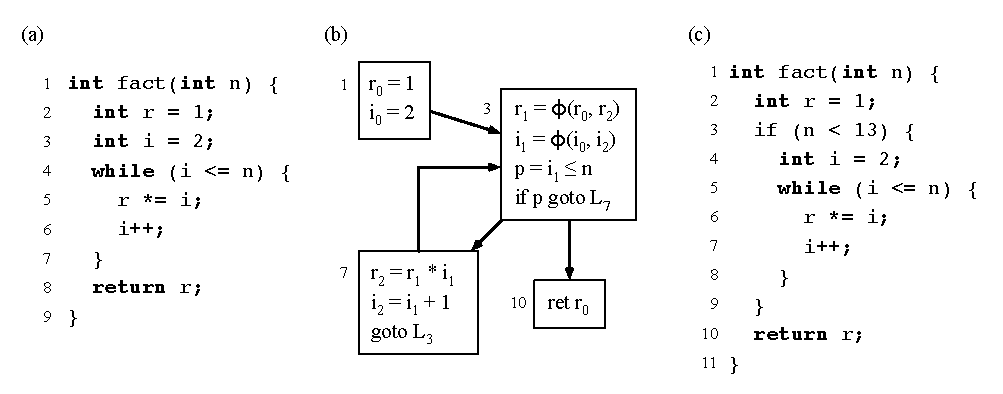
\includegraphics[width=1\textwidth]{images/fact}
\caption{(a) Uma função em C, que calcula o fatorial de um número inteiro.
(b) O CFG da função \texttt{fact}.
(c) Exemplo de laço cuja condição de parada depende de valores de entrada
mas que sempre termina.}
\label{fig:fact}
\end{center}
\end{figure}

O programa da figura~\ref{fig:fact}(a) é vulnerável a ataques de
não-terminação.
Para explicitar tal fato, a figura~\ref{fig:fact}(b) mostra o grafo de
fluxo de controle do programa.
Esse CFG está convertido para o formato de atribuição estática única
(SSA)~\cite{Cytron91}.
Usaremos essa representação de programas porque ela facilita a nossa análise
de dependência de dados.
Os blocos básicos que começam nos rótulos 3 e 7 formam um laço natural,
segundo a definição de Appel e Palsberg.
Esse laço é controlado pela condição de parada $i_1 \leq n$.
A variável $n$, o limite do laço, é dependente da entrada.
Existe um valor de $n$, a saber $\mathit{MAX\_INT}$, que força o laço a
não-terminar.

%mmmmmmmmmmmmmmmmmmmmmmmmmmmmmmmmmmmmmmmmmmmmmmmmmmmmmmmmmmmmmmmmmmmmmmmmmmmmmm
\section{Detecção e Prevenção de Não-Terminações}
\label{sec:sol}

Nesta seção descreveremos nossa técnica para detectar vulnerabilidades de
não-terminação.
Esse algoritmo de detecção fornece os subsídios necessários a uma segunda
técnica que introduzimos neste artigo: o {\em saneamento de laços}.

\subsection{Detecção Automática de Não-Terminação}
\label{sub:det}

Dizemos que um laço é {\em alcançável} quando as condições que o controlam
usam valores que dependem de dados de entrada do programa.
Note que um laço alcançável não é necessariamente vulnerável.
A título de exemplo, o programa da Figura~\ref{fig:fact}(c), uma sutil
alteração da função \texttt{fact} inicialmente vista na
figura~\ref{fig:fact}(a), termina para qualquer entrada, embora ele contenha
um laço alcançável.
Utilizamos o {\em grafo de dependências de dados} para determinar laços
alcançáveis.
Esse grafo é definido da seguinte forma:
para cada variável $v$ no programa, nós criamos um nodo $n_v$, e para cada
instrução $i$ no programa, nós criamos um nodo $n_i$.
Para cada instrução $i: v = f(\ldots, u, \ldots)$ que define uma variável $v$ e
usa uma variável $u$ n\'{o}s criamos duas areastas: $n_u \leftarrow n_i$ e
$n_i \leftarrow n_v$.
O grafo de dependências que extraímos a partir d CFG visto na
figura~\ref{fig:fact}(b) é mostrado na figura~\ref{fig:depGraph}.

\begin{figure}[t!]
\begin{center}
%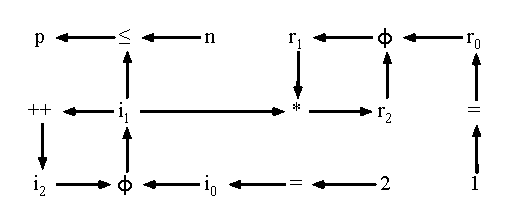
\includegraphics[width=1\textwidth]{images/depGraph}
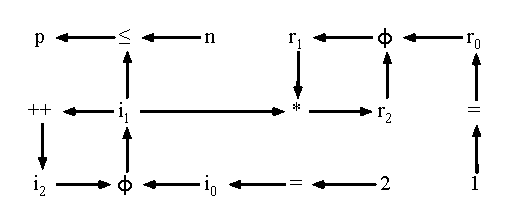
\includegraphics{images/depGraph}
\caption{(a) Grafo de dependências da função \texttt{fact}, construído a
partir do CFG visto na figura~\ref{fig:fact}(b).}
\label{fig:depGraph}
\end{center}
\end{figure}

Um caminho entre uma entrada do programa, e o predicado que controla o laço é
uma condição necessária para um ataque de não-terminação.
O grafo de dependências de nosso exemplo apresenta tal condição:
existe um caminho que une o nodo correspondente ao parâmetro \texttt{n}, uma
entrada, ao nodo que corresponde a \texttt{p}, o predicado de controle do
laço.
Esse tipo de caminho, uma vez contruído o grafo, pode ser encontrado em
tempo linear no número de arestas do grafo - normalmente proporcional ao
número de nodos - via a simples busca em profundidade ou largura.

Diremos que um laço é {\em vulnerável} quando ele é alcançável, e, além disso,
sua condição de parada é dependente de alguma operação {\em cíclica}
passível de estouro de precisão.
Seguindo a definição de laços de Appel e Palsberg, uma operação cíclica é
qualquer instrução que ocorre no corpo $S$ do laço.
Por exemplo, no CFG da figura~\ref{fig:fact}(b), as instruções
$i_2 = i_1 + 1$ e $r_2 = r_1 \times i_1$ são cíclicas.
O laço daquele exemplo encaixa-se em nossa definição de vulnerabilidade,
pois sua condição de parada é alcançável a partir da entrada, e depende de
uma instrução cíclica passível de estouro de precisão: $i_2 = i_1 + 1$.

A nossa definição de vulnerabilidade inclui muitos laços que não são
concretamente vulneráveis, tais como aquele visto na figura~\ref{fig:fact}(c).
Seria possível utilizar técnicas computacionalmente intensivas, tais como
algoritmos de satisfabilidade, para refinar a nossa definição, eliminando
alguns desses falsos positivos.
Tal abordagem já foi utilizada em trabalhos anteriores ao
nosso~\cite{Brockschmidt11,Burnim09,Gupta08,Son11,Velroyen08}.
Por outro lado, os próprios autores desses trabalhos reportam que dificilmente
suas técnicas poderiam lidar com programas muito grandes.
Nós optamos por usar uma definição mais conservadora de laço vulnerável para
termos uma ferramenta prática.
Nós sanearemos todo laço considerado perigoso, inclusive aqueles que, devido
à nossa definição liberal de vulnerabilidade, de fato não o são.
Ainda assim, conforme mostraremos na seção~\ref{sec:exp}, o impacto dessa
instrumentação é negligível.

\subsection{Saneamento de Laços}
\label{sub:san}

Uma vez encontrado um caminho vulnerável, passamos à fase de saneamento de
laços.
Um laço pode ser saneado via a inserção de testes que detectam e tratam a
ocorrência de estouros de precisão inteira.
Nós inserimos tais testes sobre as operações aritméticas cíclicas que
controlam a condição de parada do laço.
Continuando com o nosso exemplo, o laço alvo possui dois blocos básicos:
o primeiro começa no rótulo três, e o segundo começa no rótulo sete.
O laço possui duas operações aritméticas cíclicas, todas ocorrendo no segundo
bloco básico.
Dentre essas operações, aquela no rótulo sete é inofensiva: ela define a
variável $r_2$, que não participa da condição de parada do laço.
Por outro lado, a operação no rótulo oito, que define a variável $i_2$, é
usada no cálculo daquela condição, e precisa ser instrumentada.

Novamente, o grafo de dependências ajuda-nos a encontrar quais operações
precisam ser instrumentadas para sanear um laço controlado por um
predicado $p$.
Nesse caso, usamos o seguinte critério para determinar se uma operação
$i : v = f(v_1, \ldots, v_n)$ precisa ser instrumentada:
%
\begin{itemize}
\item existe um caminho no nodo $n_i$ até o nodo $n_p$.
\item O nodo $n_i$ encontra-se em um ciclo.
\end{itemize}
%
A título de exemplo, a operação de incremento $++$ no grafo de dependências
visto na figura~\ref{fig:depGraph} precisa ser instrumentada.
Em primeiro lugar, porque essa operação encontra-se em um ciclo.
Em segundo lugar, porque existe um caminho do nodo $n_{++}$ até o nodo
$n_p$.

\paragraph{Instrumentação de Saneamento. }
Para evitar que estouros de precisão venham a causar a não-terminação
de laços, nós inserimos testes no código binário do programa alvo.
O código que constitui cada um desses testes é formado por uma guarda, mas
um tratador de eventos.
Nossas guardas usam as condições mostradas na figura~\ref{fig:ovfCheck} para
verificar a ocorrência de estouros de precisão.
Atualmente instrumentamos quatro tipos diferentes de instrução:
adição, subtração, multiplicação e arredamentos para a esquerda.
As operações de adição, subtração e multiplicação podem ser com ou sem sinal
aritmético.

\begin{figure}[t!]
\begin{center}
\begin{tabular}{ll}
Instrução & Verificação \\ \\
$x = o_1 \ +_s \ o_2$ & $(o_1 > 0 \wedge o_2 > 0 \wedge x < 0) \ \ \vee$ \\
                      & $(o_1 < 0 \wedge o_2 < 0 \wedge x > 0)$ \\ \\
$x = o_1 \ +_u \ o_2$ & $x < o_1 \vee x < o_2$ \\ \\
$x = o_1 \ -_s \ o_2$ & $(o_1 < 0 \vee o_2 > 0 \vee x > 0) \ \ \vee$ \\
                      & $(o_1 > 0 \vee o_2 < 0 \vee x < 0)$ \\ \\
$x = o_1 \ -_u \ o_2$ & $o_1 < o_2$ \\ \\
$x = o_1 \ \times_{u/s} \ o_2$ & $x \neq 0 \Rightarrow x \div o_1 \neq o_2$ \\ \\
$x = o_1 \ \qside \ n$ & $(o_1 > 0 \wedge x < o_1) \vee (o_1 < 0 \wedge n \neq 0)$ \\ \\
$x = \ \downarrow_n \ o_1$ & $\mbox{cast}(x, \mbox{type}(o_1)) \neq o_1$ \\
\end{tabular}
\end{center}
\caption{\label{fig:ovfCheck}Overflow checks. Usamos $\downarrow_n$ para
descrever a operação que trunca em $n$ bits.
O subscrito $s$ indica uma operação aritmética com sinal, e o subscrito $u$
indica uma operação sem sinal.}
\end{figure}

Os testes são implementados como sequências de operações binárias, executados
logo após a instrução guardada.
Para ilustrar esse ponto, mostramos, na figura~\ref{fig:instrumented_cfg},
o código necessário para instrumentar uma soma com sinal de duas variáveis.
Essa figura mostra código no formato intermediário usado por LLVM, o compilador
que utilizamos para implementar as idéias descritas neste artigo.
Omitimos, nesse exemplo, o código do tratador de evento de estouro, pois ele
simplesmente invoca uma rotina implementada em uma biblioteca
dinamicamente compartilhada.
Conforme podemos observar pela figura, uma guarda aumenta o código instrumentado
substancialmente.
Nesse exemplo em particular a verificação requer a inserção de 14 novas
instruções no programa guardado.
Embora tal crescimento a princípio possa parecer proibitivamente grande,
os experimentos que mostraremos na seção~\ref{sec:exp} indicam que somente
uma parcela muito pequena das instruções do programa alvo precisam ser
guardadas.
Consequentemente, o custo, em termos de crescimento de código e perda de
desempenho, é negligível.

\begin{figure}[t!]
\begin{center}
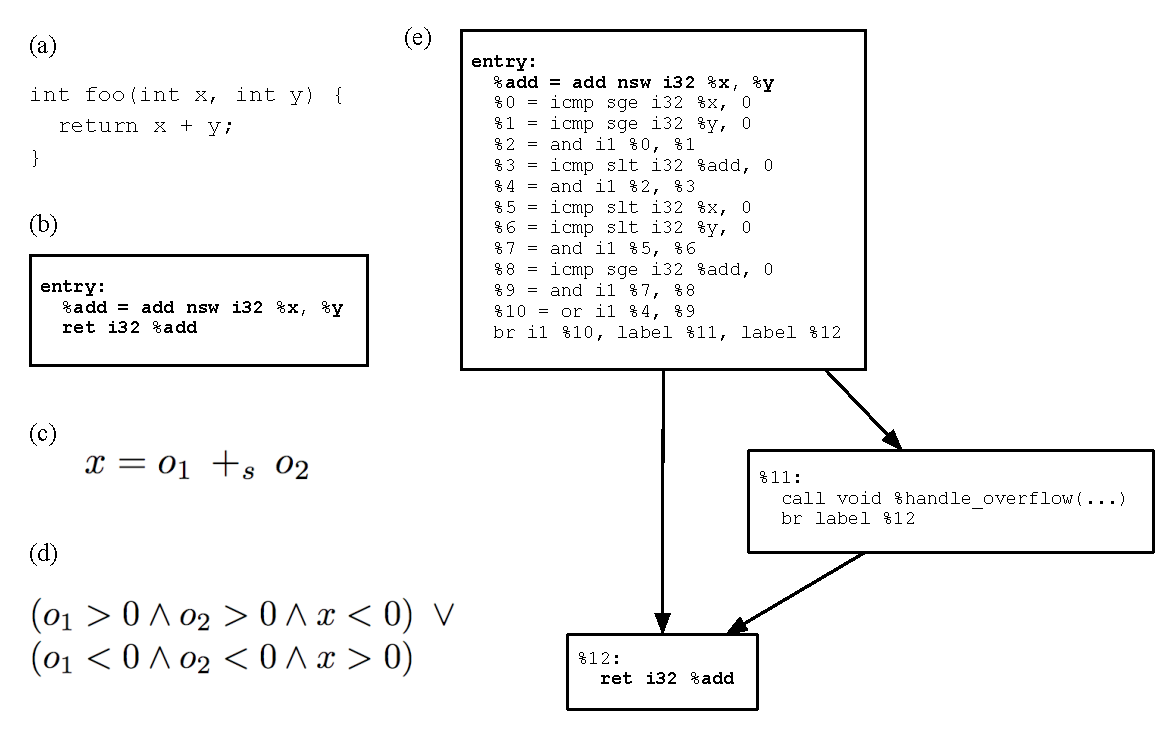
\includegraphics[width=1\textwidth]{images/instrumented_cfg}
\caption{(a) Programa que será instrumentado.
(b) Representação do programa em bytecodes LLVM.
(c) Operação que está sendo instrumentada.
(d) Teste de detecção de estouro de precisão.
(e) Programa instrumentado, em bytecodes LLVM.}
\label{fig:instrumented_cfg}
\end{center}
\end{figure}


%mmmmmmmmmmmmmmmmmmmmmmmmmmmmmmmmmmmmmmmmmmmmmmmmmmmmmmmmmmmmmmmmmmmmmmmmmmmmmm
\section{Resultados Experimentais}
\label{sec:exp}

Nós implementamos as técnicas descritas neste artigo em LLVM versão X.X.
Nossa implementação foi testada em uma máquina Intel XX, com XX Gigabtyes de
RAM, e XX GHz de Clock.
Executamos nossa análise com sucesso sobre o arcabouço de testes de LLVM,
um conjunto de programas com mais de 4.3 milhões de linhas de código C.
No restante desta seção mostraremos somente resultados obtidos sobre os
programas de SPEC CPU 2006.

\noindent
\textbf{Definição de Entrada de Dados: } nos experimentos apresentados nesta
seção, consideraremos como entrada de dados os seguintes valores:
\begin{itemize}
\item os argumentos do método \texttt{main}, isto é, as variáveis \texttt{argc}
e \texttt{argv};
\item o resultado retornado por funções {\em externas};
\item ponteiros passados como argumento de funções {\em externas}.
\end{itemize}
As funções externas são a união dos seguintes três conjuntos:
\begin{itemize}
\item funções que não foram declaradas em nenhum dos arquivos que compõem
o programa compilado;
\item funções sem corpo;
\item funções que podem ser chamadas via um ponteiro de funções.
\end{itemize}

\paragraph{Laços Alcançáveis e Vulneráveis. }
A figura~\ref{fig:staticLoopData} mostra a quantidade de laços alcançáveis e
vulneráveis que encontramos por programa.
Estamos considerando, nesse caso, somente dependências de dados que não
envolvam memória.
Em outras palavras, todos os nodos do grafo de dependência são valores que
podem residir em registradores.
Essa versão de nosso detector não é segura: podemos deixar de marcar alguns
laços vulneráveis que são controlados por dado contaminado que tenha sido
armazenado em memória.
Por outro lado, ela nos dá um número mínimo de laços que precisaríamos marcar,
de acordo com a definição de laços alcançáveis da seção~\ref{sub:det}.
Vemos, pela figura, que entre 1.3\% e 19.3\% de todos os laços do programa
são alcançáveis.
Aproximadamente a metade dos laços alcançáveis é vulnerável.
Os laços que não são considerados vulneráveis em geral usam condições de
paradas que comparam valores via igualdade, por exemplo,
\verb^while(a[i] != '\0') {i++;}^.
A figura também reporta o tamanho médio dos caminhos vulneráveis.
Um caminho vulnerável é a sequência de instruções que precisa ser executada
para que a expressão de controle do laço seja influenciada por algum valor de
entrada.
Conforme vemos pela figura, esses caminhos são geralmente pequenos.
Os dois caminhos vulneráveis em \texttt{429.mcf}, por exemplo, possuem somente
duas instruções cada um.
Concluí-se que o desenvolvedor, ao procurar por possíveis vulnerabilidades
a ataques de não terminação, teria de ater-se a uma quantidade muito pequena
de nodos do grafo de dependência do programa.

\begin{figure}[t!]
\begin{center}
\renewcommand{\arraystretch}{1.2}
\begin{tabular*}{\textwidth}{@{\extracolsep{\fill}}|l|r|r|r|r|} \hline
Benchmark & Num. Laços & Alcançáveis & Vulneráveis &
Caminhos \\ \hline
433.milc 		&	339		&	150		&	139		&	25	\\ \hline
444.namd	 		&	490		&	444		&	409		&	9	\\ \hline
447.dealII		&	4747		&	3482		&	2653		&	12	\\ \hline
450.soplex		&	535		&	506		&	453		&	14	\\ \hline
470.lbm			&	19		&	0		&	0		&	0	\\ \hline
445.gobmk		&	1068		&	574		&	497		&	17	\\ \hline
458.sjeng		&	232		&	140		&	110		&	15	\\ \hline
462.libquantum	&	75		&	44		&	41		&	10	\\ \hline
464.h264ref		&	1624 	&	194		&	164		&	17	\\ \hline
\end{tabular*}
\end{center}
\caption{Informações estáticas inferidas pela análise de não-terminação.
{\bf Num. laços}: número de laços no programa.
{\bf Alcançáveis}: quantidade de laços que são dependentes de dados produzidos a
partir de canais de entrada.
{\bf Vulneráveis}: número de laços que preenchem nossos requisitos de
vulnerabilidade.
{\bf Caminhos}: tamanho médio do menor caminho de dependência de dados da entrada
até a operação de controle do laço.}
\label{fig:staticLoopData}
\end{figure}

A figura~\ref{fig:instImpact} mostra o impacto da instrumentação que inserimos
no tamanho do programa.
Em média, cada laço vulnerável custou-nos a criação de 1.44 guardas, como
aquela vista na figura~\ref{fig:instrumented_cfg}(e).
O aumento de tamanho do programa guardado é negligível, conforme podemos
observar na última coluna da figura~\ref{fig:instImpact}.
O maior crescimento, observado em \texttt{464.h264ref}, foi de 2.28\%.
Uma vez que o número de guardas inseridas nos programas é tão pequeno, o
crescimento de seu tempo de execução também é pequeno.
Executamos todos os programas instrumentados, passando-lhes suas entradas de
referência, conforme especificado no manual de uso de SPEC CPU 2006, e as
diferenças de tempo de execução ficaram dentro da margem de erro dos benchmarks.
Em outras palavras, não pudemos perceber quaisquer diferenças, em termos de
tempo de execução, entre os programas originais e instrumentados.

\begin{figure}[t!]
\begin{center}
\renewcommand{\arraystretch}{1.2}
\begin{tabular*}{\textwidth}{@{\extracolsep{\fill}}|l|r|r|r|r|} \hline
Benchmark & Num. Instruções & Num. Arit. & Instrumentação &
Crescimento \\ \hline
433.milc 		&	24971	&	1101		&	150		&	9.49\%	\\ \hline
444.namd	 		&	77922	&	3136		&	937		&	15.73\%	\\ \hline
447.dealII		&	483614	&	14910	&	3772		&	6.42\%	\\ \hline
450.soplex		&	67808	&	1779		&	762		&	17.63\%	\\ \hline
470.lbm			&	3788		&	1130		&	0		&	0.00\%	\\ \hline
445.gobmk		&	146298	&	11856	&	939		&	9.80\%	\\ \hline
458.sjeng		&	25473	&	2138		&	167		&	9.97\%	\\ \hline
462.libquantum	&	6562		&	593		&	66		&	14.04\%	\\ \hline
464.h264ref		&	141772	&	13398	&	469		&	4.26\%	\\ \hline
\end{tabular*}
\end{center}
\caption{Impacto da instrumentação no código saneado.
{\bf Num. Instruções}: número de instruções no benchmark.
{\bf Num. Arit}: número de instruções que podem causar estouro de precisão inteira.
{\bf Instrumentação}: quantidade de testes inseridos para sanear o programa.
{\bf Crescimento}: razão entre o tamanho do programa instrumentado e o tamanho do
programa original.}
\label{fig:instImpact}
\end{figure}


\begin{figure}[t!]
\begin{center}
\renewcommand{\arraystretch}{1.2}
\begin{tabular*}{\textwidth}{@{\extracolsep{\fill}}|l|r|r|r|r|} \hline
Benchmark & Num. Op. & Num. Var. & Num. Mem. & Num. Arestas \\ \hline
433.milc			&	24799	&	20435	&	6901		&	74599	\\ \hline
444.namd			&	78043	&	72866	&	10468	&	232792	\\ \hline
447.dealII		&	512373	&	441576	&	131986	&	1516203	\\ \hline
450.soplex		&	69861	&	56172	&	21764	&	204126	\\ \hline
470.lbm			&	3787		&	3490		&	626		&	10859	\\ \hline
445.gobmk		&	152342	&	167197	&	21146	&	458405	\\ \hline
458.sjeng		&	25169	&	26313	&	2522		&	73355	\\ \hline
462.libquantum	&	6552		&	5845		&	940		&	19142	\\ \hline
464.h264ref		&	141606	&	106292	&	45223	&	409813	\\ \hline
\end{tabular*}
\end{center}
\caption{Dados do grafo de dependência dos programas analisados}.
{\bf Num. Op.}: número de nós de operação.
{\bf Num. Var.}: número de nós de variáveis e constantes.
{\bf Num. Var.}: número de nós de memória.
{\bf Num. Arestas}: número de arestas do grafo.}
\label{fig:tblDepGraph}
\end{figure}

% Describe which programs were aborted once you tried to execute them.

%mmmmmmmmmmmmmmmmmmmmmmmmmmmmmmmmmmmmmmmmmmmmmmmmmmmmmmmmmmmmmmmmmmmmmmmmmmmmmm
\section{Trabalhos Relacionados}
\label{sec:rel}

Este trabalho aborda temas relacionados a diferentes áreas da análise estática
e dinâmica de programas, a saber: teoria de fluxo de informação, detecção de
estouros de precisão inteira e análise de não-terminação.
Além disso, este trabalho utiliza o conceito de {\em grafos de dependências},
inicialmente proposto por Ferrante {\em et al.}~\cite{Ferrante87}.
Em nosso caso, o grafo de dependência dá-nos a estrutura de dados básica sobre
a qual caminhos que levam à não-terminação podem ser encontrados.
Esses grafos, contudo, historicamente vêm se prestando a muitos outros
propósitos, como escalonamento de instruções, detecção de condições de corrida e
propagação de constantes, por exemplo.

Neste artigo usamos o grafo de dependências para rastrear o fluxo de
informação contaminada.
O rastreamento de fluxo de informação é uma grande sub-área dentro do campo de
análise estática de programas~\cite{Denning77}.
Existem duas formas principais de rastrear a informação.
Pode-se traçar o fluxo de dados a partir de operações sigilosas até entradas
que um adversário pode ler.
Esse modo de rastreamento é popularmente conhecido como detecção de vazamento
de segredos~\cite{Hammer06}.
E, no sentido inverso, pode-se traçar o fluxo de informação de entradas que
um adversário pode manipular até operações críticas dentro do
programa~\cite{Tripp09}.
Essa categoria inclui nosso trabalho, além de diversos outros tipos de
vulnerabilidades, tais como {\em Injeção de Código SQL}~\cite{Wassermann07},
{\em Injeção de Scripts}~\cite{Rimsa10} e {\em Ataques de Estouro de
Buffer}~\cite{Levy96}.

Nós instrumentamos código considerado vulnerável para detectar estouros de
precisão que podem levar à não-terminação.
Esses mesmos testes já foram usados com vários outros objetivos em trabalhos
anteriores.
O mais importante trabalho nessa área deve-se, provavelmente, a Brumley
{\em et al.}~\cite{Brumley07}.
O grupo de David Brumley desenvolveu uma ferramenta, RICH, que instrumenta
cada operação aritmética passível de estouro de precisão inteira em um programa
C.
A principal conclusão daquele trabalho foi que esse tipo de instrumentação
não compromete sobremaneira o desempenho do programa modificado.
RICH, por exemplo, aumenta o tempo de execução dos programas instrumentados
em menos que 6\% em média.
Outro trabalho importante nesse campo foi publicado por Dietz
{\em et al.}~\cite{Dietz12}.
Esse grupo implementou IOC, uma ferramenta que, assim como RICH, detecta a
ocorrência de estouros de precisão em operações aritméticas inteiras.
Porém, ao contrário de Brumley {\em et al.}, Dietz {\em et al.} usaram sua
ferramenta para desenvolver um amplo estudo sobre a ocorrência de estouros
em programas reais.
Nosso trabalho difere desses outros em propósito: estamos interessados em
prevenir ataques de não terminação; e em método: nós instrumentamos somente uma
pequena parte dos programas alvo.

Finalmente, nosso trabalho relaciona-se com outros que também procuram
detectar, estaticamente, a não-terminação de programas.
A maior parte desses trabalhos utilizam análise simbólica de código para criar
expressões que levem um laço à não terminação.
Exemplos desse tipo de pesquisa incluem os trabalhos de Burnim
{\em et al.}~\cite{Burnim09}, Brockschmidt {\em et al}~\cite{Brockschmidt11} e
Veroyen {\em et al.}~\cite{Velroyen08}.
Esses trabalhos não levam em consideração possibilidade de não-terminação
devido à estouros de precisão, tampouco procuram detectar possíveis
vulnerabilidades baseadas em negação de serviço.
Existem, contudo, trabalhos na linha de detecção de não-terminação que são
bastante próximos do nosso.

Um trabalho que prova não-terminação, mesmo em face de estouros de precisão
deve-se à Gupta {\em et al.}~\cite{Gupta08}.
Gupta, assim como os trabalhos anteriormente relacionados, utiliza análise
simbólica para provar a não-terminação de programas.
A ferramenta implementada por Gupta {\em et al.}, denominada TNT, é capaz de
encontrar uma expressão algébrica que leva um laço de programa a iterar
para sempre.
Porém, TNT não aponta quais laços podem ser controlados a partir da entrada
do programa.
Por outro lado, a ferramenta  SAFERPHP, proposta por Son
{\em et al.}~\cite{Son11} possui exatamente esse objetivo.
SAFERPHP analisa o código de programas escritos em PHP, procurando por laços
que um adversário pode controlar, com o propósito, justamente, de evitar
ataques de não-terminação.
A principal diferença entre nosso trabalho, e aquele de Son {\em et al.}, é
que, enquanto nossa ferramenta busca detectar a não-terminação devido à
estouros de precisão inteira, SAFERPHP considera a aritmética de
precisão infinita.
Além disso, tanto SAFERPHP quanto TNT utilizam execução simbólica sobre caminhos
possíveis no programa alvo.
Essa abordagem, em nossa opinião, não é prática.
Testemunho disso é o fato de tais ferramentas terem sido usadas, até a presente
data, somente para analisar programas muito pequenos.

%mmmmmmmmmmmmmmmmmmmmmmmmmmmmmmmmmmmmmmmmmmmmmmmmmmmmmmmmmmmmmmmmmmmmmmmmmmmmmm
\section{Conclusão}
\label{sec:con}

Neste artigo nós descrevemos uma forma de ataque de negação de serviço que
busca levar o programa alvo à não-terminação.
Ao contrário da literatura relacionada, ate-mo-nos a ataques baseados em
estouro de precisão de aritmética de inteiros.
Esse tipo de fenômeno caracteriza linguagens de programação como Java, C e
C++.
Nós definimos algumas propriedades necessárias para a efetiva realização de
um ataque de não-terminação, a saber, condição de controle controlada por
adversário, e por operações cíclicas passíveis de estouro de precisão.
Em seguida, mostramos como eliminar a última dessas condições via guardas
inseridas pelo compilador.
Finalmente, mostramos experimentalmente que nossas guardas, ainda que inseridas
conservadoramente, não comprometem o tempo de execução do programa
instrumentado.
Demonstramos assim que a prevenção de ataques de não-terminação baseados em
estouros de precisão é barata e efetiva.

Neste trabalho nós adotamos uma definição muito conservadora de laços
vulneráveis.
De fato, muitos dos laços que indicamos como vulneráveis, em nossos
experimentos, de fato não o são.
Nossa decisão foi fruto de um compromisso entre a precisão e a eficiência:
instrumentamos todos os laços possivelmente vulneráveis, mesmo aqueles que
não são perigosos, e ainda assim mantivemos estável o tempo de execução dos
programas.
Por outro lado, é nossa intenção, em trabalho futuro, estreitar essa definição
de laço vulnerável, a fim de fornecer a desenvolvedores uma ferramenta que lhes
auxilie na descoberta de exemplos de vulnerabilidades.

\noindent
\textbf{Software: } nossas técnicas foram todas implementadas em LLVM, e estão
disponíveis publicamente na URL \texttt{http://code.google.com/p/range-analysis/}.

\bibliographystyle{plain}
\bibliography{references}

\end{document}
